\begin{frame}
	\frametitle{Neal's Algorithm 8}
	\begin{itemize}
	    %\item Markov chain with permanent state $\textbf c$ and $\boldsymbol\phi$ %(?)
		\item \textbf{Gibbs sampling} to the state extended by the addition of $m$ \textbf{auxiliary parameters} \\
		    % No integration with respect $G_{0}$ is required
        \begin{center}
        	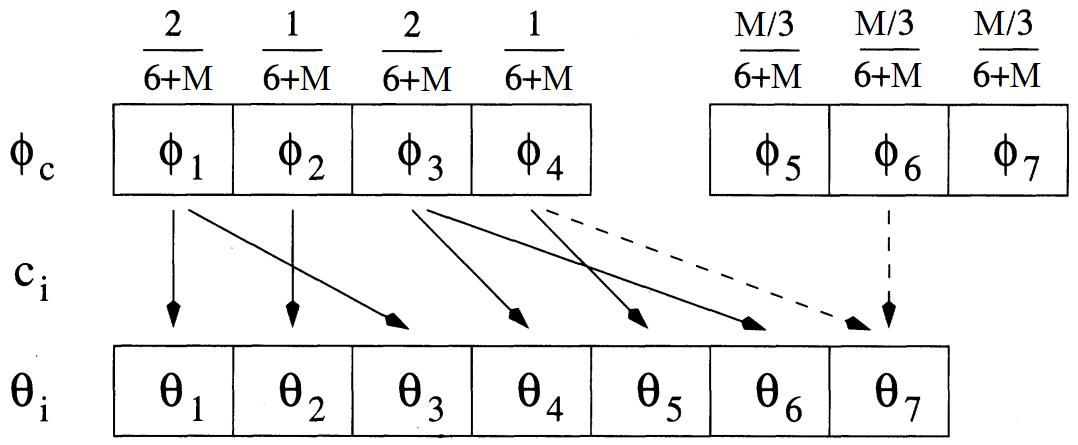
\includegraphics[scale=0.35]{etc/neal8.png}
        \end{center}
		
        \item Prior for $c_{i}$:
            \begin{align*}
            \hspace{-25pt}
            \vspace{-12pt}
                \text{If $c=c_j$ for some $j$: } \PP(c_{i}=c | c_{-i}) &= \frac{n_{-i,c}}{n-1-M}  \\
                \PP(c_{i}\neq c_{j} \text{ for all } j) &=\frac{M }{n-1-M}  \Rightarrow 
                \begin{tabular}{c}
                \textbf{split} among the $m$ \\
                auxiliary parameters 
                \end{tabular}
            \end{align*}	
	\end{itemize}
\end{frame}


\begin{frame}
	\frametitle{Neal's Algorithm 8}
	Algorithm:
		\begin{itemize}
		    \item For $i= 1,\dots,n$: update $c_{i}$
		        \begin{itemize}
		            \item Sample auxiliary parameters: \begin{list}{$\circ$}{} 
		                \item $c_{i}=c_{j}$ for some $j\ \Rightarrow$ no connection \\
		                \item $c_{i}\neq c_{j} \ \Rightarrow$ association to one of $m$
		            \end{list}

		            The other $\phi$ values drawn from $G_{0}$
		            \item Draw $c_{i}$ as follows: %(by evaluating relative prob of these possibilities)
		            	\begin{displaymath}
		            	\hspace{-20pt}
		            	P(c_{i}=c | c_{-i}, y_{i}, \phi_{1},...,\phi_{h}) \propto \begin{cases}  \frac{n_{-i,c}}{n-1-M}F(y_{i},\phi_{c}), & \mbox{for } 1 \leq c \leq k^{-} \\ \frac{M/m}{n-1-M}F(y_{i},\phi_{c}), & \mbox{for } k^{-}+1 < c \leq h
		            	\end{cases}
		            	\end{displaymath}
                    \item Discard $\boldsymbol\phi$ values not associated to any cluster
                    
                \end{itemize} 
        
            \item For $c \in \{c_{1},..,c_{n}\}$: update $\phi_{c}$ given $y_{i}$ such that $c_{i}=c$
		\end{itemize}
\end{frame}


\begin{frame}
	\frametitle{Advantages}
	\begin{itemize}
	    \item  Models with non-conjugate priors
	    \item As $m \rightarrow +\infty$ it approaches Algorithm 2 but equilibrium distribution is exact 
	    \item More efficient than similar algorithms (e.g. no-gaps) %not reduced prob to create new cluster
	    \item Hierarchical extensions
	\end{itemize}

		
\end{frame}

	

\begin{frame}
	\frametitle{Stick-Breaking Priors}
	\vspace{-15pt}
	\begin{align*}
		\mathscr{P}(\cdot)= \sum\limits_{k=1}^N
		\mathit{p_{k}}\delta_{Z_{k}}(\cdot) \\
		\mathit{p_{k}}=V_{1} \ \text{and} \  \mathit{p_{k}}=(1-V_{1})(1-V_{2}) \cdot \cdot \cdot(1-V_{k-1})V_{k} \\
		\mathbf{Z_{k}}  \iidsim H \\
		V_{k}  \iidsim Beta(a_{k},b_{k}) \\
		\mathbf{a}=(a_{1},a_{2},...) \ \text{and} \  \mathbf{b}=(b_{1},b_{2},...) \\
		0\leq\mathit{p_{k}}\leq1 \ \text{and} \ \sum\limits_{k=1}^N\mathit{p_{k}}=1 
	\end{align*}
	\vspace{-15pt}
	
	    	\begin{itemize}
	    	    \item $N<+\infty$: \ $\mathscr{P}_{N}(\textbf{a},\textbf{b})$
	    	    \begin{itemize}
	    	        \item $\mathbf{p} \sim \mathscr{GD}(\textbf{a},\textbf{b})$
	    	        \item e.g. all finite dimensional Dirichlet priors
	    	    \end{itemize}
	    	    \item $N=+\infty$: $\mathscr{P}_{\infty}(\textbf{a},\textbf{b})$
	    	    \begin{itemize}
	    	        \item e.g. Dirichlet process, the two parameter Poisson-Dirichlet process
	    	    \end{itemize}
	    	\end{itemize}
\end{frame}


\begin{frame}
	\frametitle{Blocked Gibbs Algorithm}
	\begin{itemize}
	    \item Assumption: \textbf{finite-dimensional} prior  $P \sim  \mathscr{P}_{N}(\textbf{a},\textbf{b})$
	
%(main use: approximate DPMmodels by truncating the stick-breaking representation of the DP)\\
        \item Finite number of variables $\Rightarrow$ \textit{blocks of parameters} \\
        \item \textbf{Model}:\\
        \begin{align*}
            (Y_{i}|\mathbf{\phi},\mathbf{c})&\indsim F(\phi_{c_{i}}) , \ i=1,..,n \\
            (c_{i}|\mathbf{p})&\iidsim\sum\limits_{k=1}^N \mathit{p_{k}}\delta_{k}(\cdot)\\
            \mathbf{p} &\sim \mathscr{GD}(\textbf{a},\textbf{b}) \\
            \mathbf{\phi}_{c} & \sim G_{0}
        \end{align*}



	\end{itemize}
\end{frame}




\begin{frame}
	\frametitle{Blocked Gibbs Algorithm}
	Algorithm: \\
	Repeatedly drawing values from conditional distributions of the blocked variables

	\begin{itemize}
    	\item $(\phi | \textbf{c}, \textbf{Y})$
	    \item $(\textbf{c}| \phi,\textbf{p}, \textbf{Y})$
    	\item $(\textbf{p}| \textbf{c})$
	\end{itemize}

	\textbf{Direct sampling of the posterior} $\mathscr{P}(\cdot|\mathbf{Y})$ :\\

	\begin{itemize}
    	\item The Algorithm produces draws from $(\phi,\textbf{c},\textbf{p}| \textbf{Y})$ \\
		\item Each draw $(\phi,\textbf{c},\textbf{p})$ defines a measure $P(\cdot)= \sum\limits_{k=1}^N  \mathit{p_{k}}\delta_{\phi_{k}}(\cdot) $
		\item Each $P$ is a drawn from $\mathscr{P}(\cdot|\mathbf{Y})$
	\end{itemize}
\end{frame}

\begin{frame}
	\frametitle{Advantages}
		\begin{itemize}
		     \item Handles the issue of conjugacy
	   	    	% nonconjugate case Metropolis–Hastings for phi
		    \item Good mixing %(block)
		    \item Hierarchical extensions
	\end{itemize}

\begin{frame}
	\frametitle{Code structure}
	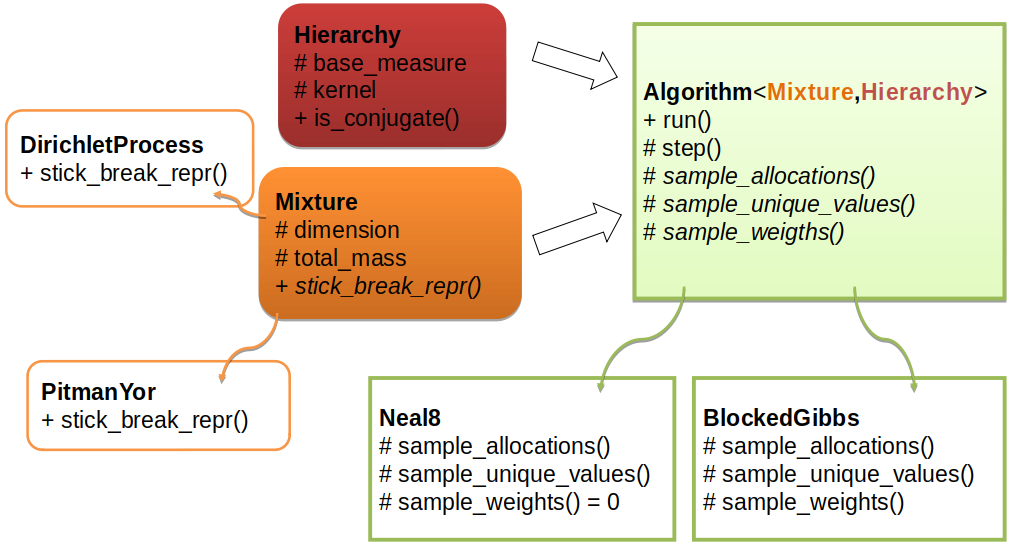
\includegraphics{etc/code_map.png}
\end{frame}

\end{frame}

